\documentclass[12pt,a4paper]{article}
\usepackage{vmargin}
\setmarginsrb{1.0in}{1.0in}{1.0in}{1.0in}{0mm}{0mm}{0mm}{10mm}

\usepackage{amsfonts,amsmath,amssymb}
\usepackage{amsthm}
\usepackage{graphicx}
\usepackage{amsmath}
\usepackage{xcolor}
%\usepackage{ngerman}
\usepackage{listings}
\usepackage[utf8]{inputenc}
%\usepackage[T1]{fontenc}
\usepackage{comment}
\usepackage{algorithm}
\usepackage{hyperref}
%%\usepackage{algpseudocode}
\renewcommand*\thealgorithm{}
\usepackage{algorithmic}
\usepackage{amsmath}

\newcommand{\N}{\mathbb{N}}
\newcommand{\R}{\mathbb{R}}
\renewcommand{\O}{\mathcal{O}}
\usepackage{mathtools}

\newtheorem{theorem}{Theorem}
\newtheorem{lemma}{Lemma}
\newtheorem{corollary}[theorem]{Corollary}
\newtheorem{conjecture}{Conjecture}
\newtheorem{fact}[theorem]{Fact}
%\newtheorem{proposition}[theorem]{Proposition}
\newtheorem{observation}{Observation}
%\newtheorem{notation}[theorem]{Notation}
\newtheorem{remark}{Remark}
\newtheorem{claim}{Claim}
\newtheorem{definition}{Definition}
%\theoremstyle{definition}
%\newtheorem{problem}[theorem]{Problem}
\newtheorem{example}{Example}
%\renewcommand{\qedsymbol}{\rule{1mm}{1mm}}
\newcommand\independent{\protect\mathpalette{\protect\independenT}{\perp}}
\def\thesection{\alph{section}}

\setlength{\parindent}{0pt}


\begin{document}

\noindent
\begin{minipage}{0.66\textwidth}
Hasso Plattner Institute Potsdam\\
\\
Seminar on Nature Inspired Algorithms\\ Summer 2017\\
Potsdam, \today
\end{minipage}
~
\begin{minipage}{0.30\textwidth}

\includegraphics[width=\textwidth]{../homework_template/Hasso_Plattner_Institut_Logo}
\end{minipage}


\begin{center}
 {\LARGE \textbf{Homework 3}\\ \small Willi Gierke}
 \vspace*{0.5cm}
\end{center}
%%%%%%%%%%%%%%%%%%%%%%%%%%%%%%%%%%%%%%%%%%%


\includegraphics[clip, trim=0.5cm 2.5cm 0.5cm 4cm, width=0.99\textwidth, page=2]{homework03.pdf}
\clearpage
\section{}
The expected run time of \textsc{RandomSearch} is
\begin{align*}
E(T_{RS}) \in \mathcal{O}(2^n).
\end{align*}
It does not take $g$ into account but only looks at some random mutation of a bitstring in each iteration. The chance of getting the all-1s-bitstring is $\frac{1}{2^n}$ which gives us the above run time.


\section{}
The probability of the event X of a string with at most  $n/4$ zeros is equal to the probability of having more than  $3n/4$ ones. We can estimate this probability using Markov's Inequality:
\begin{center}

 $Pr(X \geq a) \leq \frac{E(X)}{a}$\\
 \bigskip
 let $E(X) = \frac{n}{2} \implies Pr(X \geq (3n/4)) \leq \frac{n/2}{3n/4} = \frac{n}{2} * \frac{4}{3n} = \frac{2}{3} $ \\
 \bigskip
 $\implies Pr(X) \leq \frac{2}{3}$

%  $$p_i = 1/2, E(X) = n/2, \text{fix } \delta = 1/2 \rightarrow (1 + \delta)E(X)=(3/4)n$$
%  $$Pr(\mathcal{E}) = Pr(X > (3/4)n) \leq \Bigg(\frac{e^{1/2}}{(3/2)^{(3/2)}}\Bigg)^{n/2}$$
\end{center}

\section{}
To reach the optimum from a solution after $\mathcal{E}$ did not occur, we need to flip at least $n/4+1$ zeros without flipping the remaining ones.
\begin{align*}
 P(Optimum|\neg\mathcal{E}) &\leq \Big(\frac{1}{n}\Big)^{n/4+1} \Big(1-\frac{1}{n}\Big)^{3n/4-1} \\
 &= \Big(\frac{1}{n}\Big) \Big(\frac{1}{n}\Big)^{n/4} \Big(\frac{n-1}{n}\Big)^{3n/4-1} \\
 &= \Big(\frac{1}{n}\Big) \Big(\frac{1}{n}\Big)^{n/4} \Big(\frac{n-1}{n}\Big)^{3n/4}\Big(\frac{n-1}{n}\Big)^{-1} \\
 &= \Big(\frac{1}{n-1}\Big) \Big(\frac{1}{n}\Big)^{n/4} \Big(\frac{n-1}{n}\Big)^{3n/4} \\
\end{align*}
The expected run time is the inverse of the probability.
\begin{align*}
 E(T_{1+1}|\neg \mathcal{E}) &\geq (n-1) \Big(\frac{1}{n}\Big)^{-n/4} \Big(\frac{n-1}{n}\Big)^{-3n/4} \\
  &= (n-1)\ n^{n/4}\ (n-1)^{-3n/4}\ n^{3n/4} \\
  &= (n-1)^{1-(3n/4)}\ n^{n} \\
\end{align*}

\section{}
\begin{align*}
E(T_{RS})&=\mathcal{O}(2^n)\\
E(T_{1+1})&=E(T|\mathcal{E})Pr(\mathcal{E}) + E(T|\neg \mathcal{E})Pr(\neg \mathcal{E})\\
\end{align*}
We only  look at the second part the equation, i.e. $E(T|\neg \mathcal{E})Pr(\neg \mathcal{E})$. The first part cannot become negative, so it will only increase the expected run time. We use $Pr(\neg \mathcal{E})$ from task $b$ and $E(T|\neg \mathcal{E})$ from task $c$. We follow
\begin{align*}
 E(T|\neg \mathcal{E})Pr(\neg \mathcal{E})& \geq
 (n-1)^{1-3n/4} n^{n} \Bigg(1-\Big(\frac{2}{3}\Big)\Bigg)\\
\end{align*}
To prove that the run time of \textsc{1+1 EA} is worse than the one of \textsc{RandomSearch}, we divide the expected run time of 1+1 EA by the one of \textsc{RandomSearch} and show that the quotient goes to infinity when $n$ goes to infinity. \begin{align*}
 \frac{E(T_{1+1})}{E(T_{RS})} &= \frac{\frac{1}{3}(n-1)^{1-3n/4}\ n^{n}}{2^n} \\
 &= \frac{1}{3}(n-1)^{1-3n/4}\ \Big(\frac{n}{2}\Big)^n \\
 \lim_{n\to\infty} (n-1)^{1-3n/4}\Big(\frac{n}{2}\Big)^n &= \infty
\end{align*}

As this goes to infinty, we can see that 1+1 EA has a worse expected runtime than \textsc{RandomSearch}.


\end{document}
